\section{应用：连续时间随机逼近}
\label{sec:ctsp-stochastic-approximation}

上一节的采样过程要长期保持一个非退化的分布：噪声不能消失，否则过程会停在势函数的最低点，而不是遍历整个目标。本节的任务相反。第~\ref{chap:discrete-time-stochastic-processes}章的Robbins--Monro递推只能观察到带噪声的响应，却要逼近方程$h(\bm\theta)=\bm0$的根；它让步长逐渐减小，使噪声的影响越来越弱，最终把迭代钉在根上。这里把这个机制放到连续时间：观测是连续到达的带噪信号，增益随时间递减，问题是状态是否收敛到指定的零点。

\subsection{连续观测与递减增益}
\label{sec:ctsp-sa-setting}

\paragraph{从离散递推到连续观测}
离散的随机逼近写成$\bm\theta_{n+1}=\bm\theta_n+a_n[h(\bm\theta_n)+\bm\xi_{n+1}]$：平均漂移$h$把迭代推向根，鞅差$\bm\xi_{n+1}$是观测噪声，步长$a_n$满足$\sum a_n=\infty$、$\sum a_n^2<\infty$。连续时间中，带噪响应以信号的形式到达：设观测过程满足
\begin{equation}
  \mathrm d\bm Y_t=h(\bm\theta_t)\,\mathrm dt+\bm\sigma(\bm\theta_t)\,\mathrm d\bm W_t ,
  \label{eq:ctsp-sa-observation}
\end{equation}
每段短时间内观测到的增量$\mathrm d\bm Y_t$是当前参数下平均响应的$\mathrm dt$倍，叠加一个Brownian噪声。增益为$a(t)>0$的连续随机逼近按观测调整参数：
\begin{equation}
  \mathrm d\bm\theta_t=a(t)\,\mathrm d\bm Y_t=a(t)h(\bm\theta_t)\,\mathrm dt+a(t)\bm\sigma(\bm\theta_t)\,\mathrm d\bm W_t .
  \label{eq:ctsp-continuous-sa}
\end{equation}
与离散情形一样，算法使用的是观测$\mathrm d\bm Y$，并不需要能直接计算$h$；$h$与$\bm\sigma$只在分析中出现。

\paragraph{增益条件的含义}
本节取确定的、连续的正增益$a(t)$，常用的例子是$a(t)=1/(1+t)$。离散步长的两个条件在连续时间中对应
\begin{equation}
  \int_0^\infty a(t)\,\mathrm dt=\infty,\qquad\int_0^\infty a(t)^2\,\mathrm dt<\infty .
  \label{eq:ctsp-gain-conditions}
\end{equation}
第一个条件保留累计调整能力：确定性部分$\dot{\bm\theta}=a(t)h(\bm\theta)$走过的“路程”由$\int a\,\mathrm dt$度量，它必须是无穷，才能从任意远的初值走到根。第二个条件控制噪声：在$\bm\sigma$有界时，噪声项$\int_0^ta(s)\bm\sigma\,\mathrm d\bm W_s$的二阶矩由Itô等距等于$\int_0^ta^2\|\bm\sigma\|_{\mathrm F}^2\,\mathrm ds$，有限的总量使这个鞅$L^2$有界，从而收敛，噪声的总影响有限。$a(t)=1/(1+t)$同时满足两者；$a(t)=(1+t)^{-\beta}$在$\frac12<\beta\leq1$时满足，$\beta\leq\frac12$时噪声累计无界，$\beta>1$时调整总量有限。

增益条件只是收敛的一部分条件。还需要方程~\eqref{eq:ctsp-continuous-sa}有不爆炸的解，噪声的矩受控，并且平均漂移$h$确实把状态吸引向根。下一小节在一组可以直接检查的条件下把这些部分组合起来。

\subsection{随机Lyapunov方法与平均动力学}
\label{sec:ctsp-sa-lyapunov}

\paragraph{收敛定理}
离散章用非负误差量的几乎超鞅递推证明随机逼近收敛。连续时间的对应工具是：对误差的Lyapunov函数使用Itô公式，把漂移的下降、二阶修正和鞅项分开，再把正的二阶修正吸收进一个积分因子。

\begin{theorem}[连续时间随机逼近的收敛]
  \label{thm:ctsp-sa-convergence}
  设$h$与$\bm\sigma$全局Lipschitz，$\bm\theta^\star$满足$h(\bm\theta^\star)=\bm0$，并且存在常数$c,K>0$，使对所有$\bm\theta$，
  \[
    (\bm\theta-\bm\theta^\star)^\top h(\bm\theta)\leq-c\|\bm\theta-\bm\theta^\star\|_2^2,\qquad
    \|\bm\sigma(\bm\theta)\|_{\mathrm F}^2\leq K\bigl(1+\|\bm\theta-\bm\theta^\star\|_2^2\bigr).
  \]
  设增益$a(t)$确定、连续、为正并满足式~\eqref{eq:ctsp-gain-conditions}，初值$\bm\theta_0$确定。则$\bm\theta_t\to\bm\theta^\star$几乎必然。
\end{theorem}

\begin{proof}
系数全局Lipschitz（乘以局部有界的$a(t)$后在有限时段上仍是），定理~\ref{thm:ctsp-sde-existence}给出全时间的强解。记$V_t=\|\bm\theta_t-\bm\theta^\star\|_2^2$。由Itô公式，
\[
  \mathrm dV_t=\bigl[2a(t)(\bm\theta_t-\bm\theta^\star)^\top h(\bm\theta_t)+a(t)^2\|\bm\sigma(\bm\theta_t)\|_{\mathrm F}^2\bigr]\mathrm dt+\mathrm dM_t ,
\]
其中$M_t=\int_0^t2a(s)(\bm\theta_s-\bm\theta^\star)^\top\bm\sigma(\bm\theta_s)\,\mathrm d\bm W_s$是局部鞅。由两个假设，漂移不超过$-2caV_t+Ka^2(1+V_t)$。

正的二阶修正$Ka^2(1+V)$用积分因子吸收。令
\[
  A_t=\exp\Bigl\{-K\int_0^ta(s)^2\,\mathrm ds\Bigr\},
\]
由增益条件，$A_t$从$1$单调下降到正的极限$A_\infty$。由乘积法则（$A$有限变差），
\[
  \mathrm d\bigl[A_t(1+V_t)\bigr]=A_t\bigl[\mathrm dV_t-Ka(t)^2(1+V_t)\,\mathrm dt\bigr]\leq-2ca(t)A_tV_t\,\mathrm dt+A_t\,\mathrm dM_t .
\]
于是$S_t=A_t(1+V_t)+\int_0^t2ca(s)A_sV_s\,\mathrm ds$满足$\mathrm dS_t\leq A_t\,\mathrm dM_t$。记$L_t=S_0+\int_0^tA_s\,\mathrm dM_s$，则$L_t-S_t$非减且从零出发，所以$0\leq S_t\leq L_t$。$L$是非负局部鞅，由第~\ref{sec:ctsp-continuous-martingales}节它是超鞅；对$s\leq t$，$\mathbb E[S_t\mid\mathcal F_s]=\mathbb E[L_t\mid\mathcal F_s]-\mathbb E[L_t-S_t\mid\mathcal F_s]\leq L_s-(L_s-S_s)=S_s$，所以$S$也是非负超鞅。由定理~\ref{thm:ctsp-martingale-convergence}，$S_t$几乎必然收敛到有限极限。

$S$的两部分都非负，第二部分随$t$非减，所以二者分别收敛：$\int_0^\infty a(s)A_sV_s\,\mathrm ds<\infty$，并且$A_t(1+V_t)$收敛，再由$A_t\to A_\infty>0$得$V_t$收敛到某个$V_\infty$。若$V_\infty>0$，由$A_s\geq A_\infty$，积分$\int_0^\infty a(s)A_sV_s\,\mathrm ds$的被积函数最终不小于$\frac12a(s)A_\infty V_\infty$，而$\int a=\infty$，矛盾。所以$V_\infty=0$。
\end{proof}

证明的结构与离散章的几乎超鞅定理一一对应：$-2caV$是累计下降项，$Ka^2(1+V)$是可求和的误差项（由$\int a^2<\infty$），$M$是鞅噪声。连续时间新增的是两步：用Itô公式而不是一步展开得到漂移，以及用局部化与Fatou引理处理只是局部鞅的噪声。强单调条件可以放宽为一般的Lyapunov函数条件，但需要另外保证轨迹有界。

\paragraph{常增益的对照}
若把增益固定为常数$a$，第二个增益条件失效，噪声不再消失。以标量$h(\theta)=\mu-\theta$、常数$\sigma$为例，式~\eqref{eq:ctsp-continuous-sa}化为$\mathrm d\theta=a(\mu-\theta)\,\mathrm dt+a\sigma\,\mathrm dW$，这是一个以$\mu$为中心的OU过程，稳态方差为$(a\sigma)^2/(2a)=a\sigma^2/2$。状态在$\mu$附近持续波动，波动幅度按$\sqrt a$缩小；它跟踪得快，但不收敛。常增益适合目标会缓慢变化的情形，此时研究的是稳态波动与跟踪误差，而不是收敛。这里的方差公式依赖噪声非退化与线性结构；一般非线性情形只能给出上界，正的极限方差需要额外条件。

\paragraph{算法时钟与平均ODE}
增益递减的过程还可以换一个时钟来看。定义算法时间$s(t)=\int_0^ta(u)\,\mathrm du$，它是严格递增的连续函数，由第一个增益条件趋于无穷；记其反函数为$t(s)$，令$\widetilde{\bm\theta}_s=\bm\theta_{t(s)}$。漂移部分在新时钟下变成$h(\widetilde{\bm\theta}_s)\,\mathrm ds$，增益被吸收掉了。噪声部分需要一个时间变换的事实：$\bm B_s=\int_0^{t(s)}\sqrt{a(u)}\,\mathrm d\bm W_u$是连续鞅，二次变差为$\int_0^{t(s)}a(u)\,\mathrm du\,\bm I=s\bm I$，由Lévy的Brownian刻画它是标准Brownian运动\scite{math-kallenberg2021probability}。由$a\,\mathrm dW=\sqrt a\cdot\sqrt a\,\mathrm dW$，
\begin{equation}
  \mathrm d\widetilde{\bm\theta}_s=h(\widetilde{\bm\theta}_s)\,\mathrm ds+\sqrt{a(t(s))}\,\bm\sigma(\widetilde{\bm\theta}_s)\,\mathrm d\bm B_s .
  \label{eq:ctsp-algorithm-clock}
\end{equation}

在算法时钟下，确定性部分就是平均ODE $\dot{\bm\theta}=h(\bm\theta)$，与离散章的平均ODE方法一致；噪声的系数是$\sqrt{a(t(s))}$，随算法时间趋于零。所以长时间以后，过程在任意固定长度的算法时间窗内越来越接近平均ODE的轨迹，收敛性可以从ODE的稳定性读出。上面的定理没有走这条路，而是直接用Lyapunov函数闭合证明，因为它只需要可以逐项检查的条件。这里的时间变换只改变给定增益下的时间尺度；它说明递减增益的随机逼近为什么可以用平均ODE描述，并不意味着所有随机微分方程都是随机逼近。

\subsection{可解实例、离散实现与误差分工}
\label{sec:ctsp-sa-example}

\paragraph{连续观测下的均值估计}
最简单的例子是估计一个未知漂移。设观测为$\mathrm dY_t=\mu\,\mathrm dt+\sigma\,\mathrm dW_t$，$Y_0=0$，目标是$\mu$。取$h(\theta)=\mu-\theta$，即用观测增量减去当前估计的预测，增益$a(t)=1/(1+t)$：
\[
  \mathrm d\theta_t=\frac{\mathrm dY_t-\theta_t\,\mathrm dt}{1+t} .
\]
乘以$1+t$并用乘积法则，$\mathrm d[(1+t)\theta_t]=\theta_t\,\mathrm dt+(1+t)\,\mathrm d\theta_t=\mathrm dY_t$，所以
\begin{equation}
  \theta_t=\frac{\theta_0+Y_t}{1+t} .
  \label{eq:ctsp-sa-solution}
\end{equation}
由$Y_t=\mu t+\sigma W_t$，
\[
  \mathbb E\theta_t=\frac{\theta_0+\mu t}{1+t}=\mu+\frac{\theta_0-\mu}{1+t},\qquad
  \operatorname{Var}(\theta_t)=\frac{\sigma^2t}{(1+t)^2}.
\]
偏差按$1/t$消失，方差按$\sigma^2/t$下降，均方误差约为$\sigma^2/t$。由$W_t/t\to0$几乎必然，$\theta_t\to\mu$几乎必然，这与定理~\ref{thm:ctsp-sa-convergence}的结论一致（这里$c=1$，$K=\sigma^2$）。图~\ref{fig:ctsp-sa-paths}画出了路径束：所有路径从同一初值出发，偏差与波动同时收缩。

\begin{figure}[htbp]
  \centering
  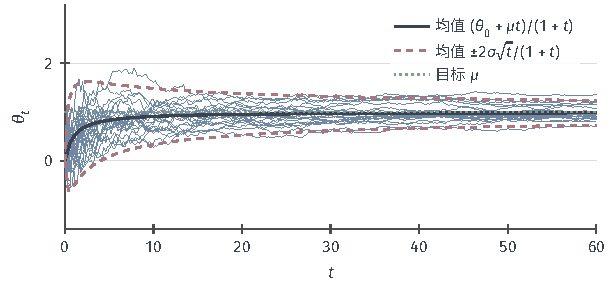
\includegraphics[width=105mm]{figures/03-optimization-evolution-and-signals/02-processes-and-trajectory-evolution/tikz/ctsp-sa-paths/figure.pdf}
  \caption{连续时间随机逼近的路径束。观测$\mathrm dY=\mu\,\mathrm dt+\sigma\,\mathrm dW$，$\mu=1$，$\sigma=1$，增益$1/(1+t)$，$\theta_0=0$；由显式解$\theta_t=(\theta_0+Y_t)/(1+t)$在网格上生成$25$条路径，固定随机种子。黑线为均值，红虚线为均值$\pm2\sigma\sqrt t/(1+t)$，绿点线为目标$\mu$。与图~\ref{fig:ctsp-ou-envelope}的OU过程不同，这里的波动带随时间收窄到零。}
  \label{fig:ctsp-sa-paths}
\end{figure}

这个例子也说明，同一个对象可以从两个角度研究。作为算法，$\theta_t$是一个随机逼近过程，我们关心它是否、以多快的速度收敛到方程的根$\mu$。作为统计量，$\theta_t\approx Y_t/t$是由连续观测估计漂移的估计量，可以继续问它在所有估计量中是否最优、渐近分布能否用来构造置信区间。前一个问题属于本节，后一个问题需要统计推断的框架，见\BookChapterRef{chap:statistical-inference}{卷四“统计推断”章}。

\paragraph{离散实现与误差分工}
在计算机上实现连续随机逼近，需要把时间离散。取步长$\Delta$，第$k$步的增益为$a_k=a(k\Delta)\Delta$，观测增量为$\Delta Y_k=Y_{(k+1)\Delta}-Y_{k\Delta}$，更新为$\theta_{k+1}=\theta_k+a(k\Delta)[\Delta Y_k-\theta_k\Delta]$。这已经是一个离散的Robbins--Monro递推，步长$a_k$满足离散的两个条件。

误差来源应当分别记录。一是增益调度的离散：$a_k$是连续增益的近似，改变了有效的算法时钟。二是时间网格：在每步内冻结$\theta$，与连续方程相差一个与$\Delta$同阶的项。三是噪声的生成：若$Y$本身是模拟的，模拟误差按第~\ref{sec:ctsp-error-types}节分析；若$Y$来自真实观测，则没有这一项。四是有限运行时间：即使离散与连续完全一致，在时刻$T$停止时仍有$\sigma^2/T$量级的随机误差。前三项属于数值计算，第四项是算法本身在有限时间内的误差。至于$\mu$能否从观测中识别、估计量是否有效，是统计问题，不在这里的误差分工之内。
